\documentclass[12pt,titlepage]{article}
\usepackage{graphicx}
\usepackage{longtable}
\author{\textbf{The TOME Team}\\
Curtis ``Fjord'' Hawthorne \\
Craig Miller\\
Clint Olson\\
fREW Schmidt
}
\title{\textbf{TOME Application Model}}
\begin{document}
\maketitle
\tableofcontents
\listoffigures
\newpage
\section{Introduction}
\subsection{Purpose of Document}
The purpose of this document is to specify the TOME system and the application model it uses.

An application is defined as having business logic and presentation elements while an individual component is defined as providing a particular set of services or presentation---but not both. This approach allows for the structure of a modern component based distributed system.

Delivery scheduling and testing issues are also dealt with to ensure that other related applications and components can be developed in parallel.
\subsection{Background}
In December of 2003, several students on Dorm 41 started a system called TOME.  The basic idea is that at the end of the semester, instead of everyone selling their books back to the bookstore, they all donate them to central repository.  Anyone on the floor can then check out whatever books they need free of charge for a semester.

The advantage of having a computer-based system to keep track of all those books is easy to see, and one has been under development ever since the start of TOME.  Since its humble beginnings as a quick solution over Christmas break, the system has grown to well over 3,000 lines of Perl code as well as HTML templates, a well-planned database schema, and significant documentation.  The system not only has comprehensive facilities for tracking books and patrons, but also keeps tabs on what books are used for what classes and other alternatives to purchasing new books.
\subsection{References}
\label{references}
All project data will be stored in a combination Subversion repository and Trac environment.  All of this will be made viewable at the following URL:

\texttt{http://enosh.letnet.net/trac/tome}
\section{Application Overview}
\subsection{Scope}
The TOME system is responsible for managing:
\begin{itemize}
	\item Books
	\item Book information
	\item Class information
	\item Class-to-book mappings
	\item Book reservations
	\item Book checkouts
\end{itemize}
The TOME system is \textbf{not} responsible for managing:
\begin{itemize}
	\item Book acquisition
	\item Book disposal
	\item Selling old books
	\item Any financial activity
\end{itemize}
\subsection{Context}
TOME exists as an independent system with no ties to other databases.  Information from other databases, such as class listings, book information, and book-to-class associations will be used, but not in an automated fashion.
\subsection{Technical Environment}
TOME is a web-based Perl application.  It is intended to be run under the Apache webserver, but any webserver that supports CGI should be capable of running the system.  Template::Toolkit is used to process HTML templates.  PostgreSQL is used as the database backend.  CGI::Application is used as the framework for the system as a whole.
\section{Actors}
\subsection{Actor Diagram}
Figure~\ref{userdiagram} shows an overview of the actors involved in the TOME system and how they interact with each other.  Patrons talk to TOMEkeepers who use the TOME web interface which is based on the TOME database.
\begin{figure}[h]
	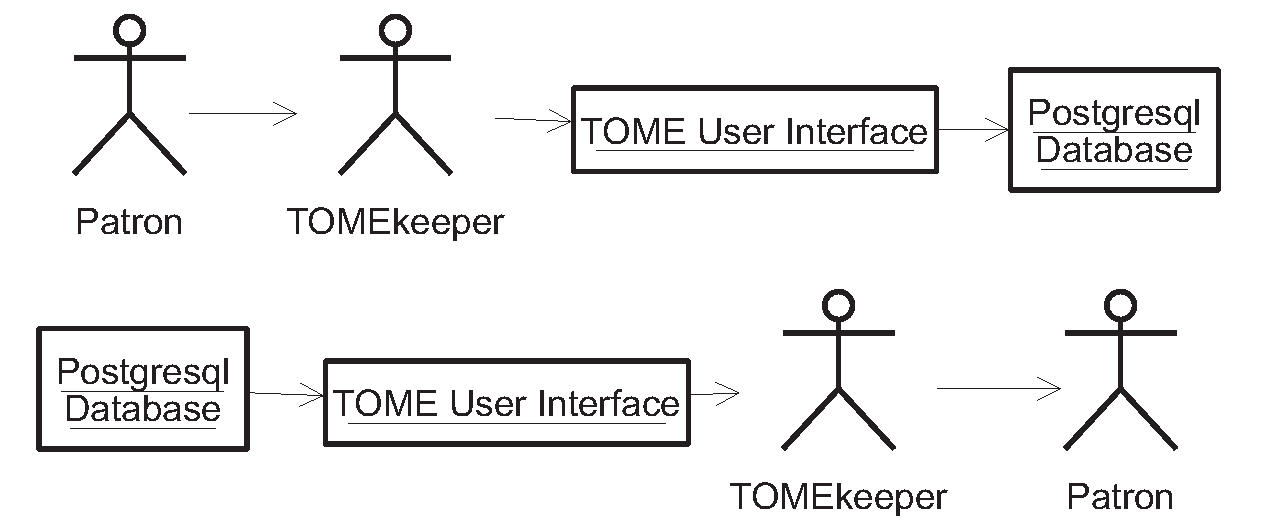
\includegraphics[width=\textwidth]{userdiagram}
	\caption{Actor Diagram}
	\label{userdiagram}
\end{figure}
\subsection{Actor Definitions}

\subsubsection{Patron}
\begin{longtable}{|p{.25\textwidth}|p{.75\textwidth}|}
	\hline
	\textbf{Description} & The Patron is any student who wishes to use the TOME system.  Only students that reside on floors with an active TOME system can become Patrons. Patrons never interact directly with TOME, only through TOMEkeepers.  \\
	\hline
	\textbf{Aliases} & Student. \\
	\hline
	\textbf{Inherits} & None. \\
	\hline
	\textbf{Actor Type} & Passive - Person. \\
	\hline
\end{longtable}

\newpage
\subsubsection{TOMEkeeper}
\begin{longtable}{|p{.25\textwidth}|p{.75\textwidth}|}
	\hline
	\textbf{Description} & The TOMEkeeper is the primary user of the TOME system.  They are responsible for all interactions with Patrons, all system administration, and all TOME activity. \\
	\hline
	\textbf{Aliases} & None. \\
	\hline
	\textbf{Inherits} & None. \\
	\hline
	\textbf{Actor Type} & Active - Person. \\
	\hline
\end{longtable}

\section{Business Use Cases}
\subsection{Use Case Listing}
\begin{longtable}{|p{.10\textwidth}|p{.40\textwidth}|p{.50\textwidth}|}
	\hline
	\textbf{ID} & \textbf{Use Case Name} & \textbf{Comments} \\
	\hline
	UC01 & Book Added & When a book is donated to the TOME system \\
	\hline
	UC02 & Book Reserved & When a patron requests that book be reserved for a particular semester \\
	\hline
	UC03 & Book Checked Out & When a patron checks out a physical book \\
	\hline
	UC04 & Class Added & When a TOMEkeeper adds a class to the system \\
	\hline
	UC05 & Book Added To Class & When a TOMEkeeper adds a book to a particular class \\
	\hline
\end{longtable}
\subsection{Graphical Use Case Diagram}
This section represents the business use cases of the TOME system in graphical form in Figure~\ref{usecase}.
\begin{figure}[h]
	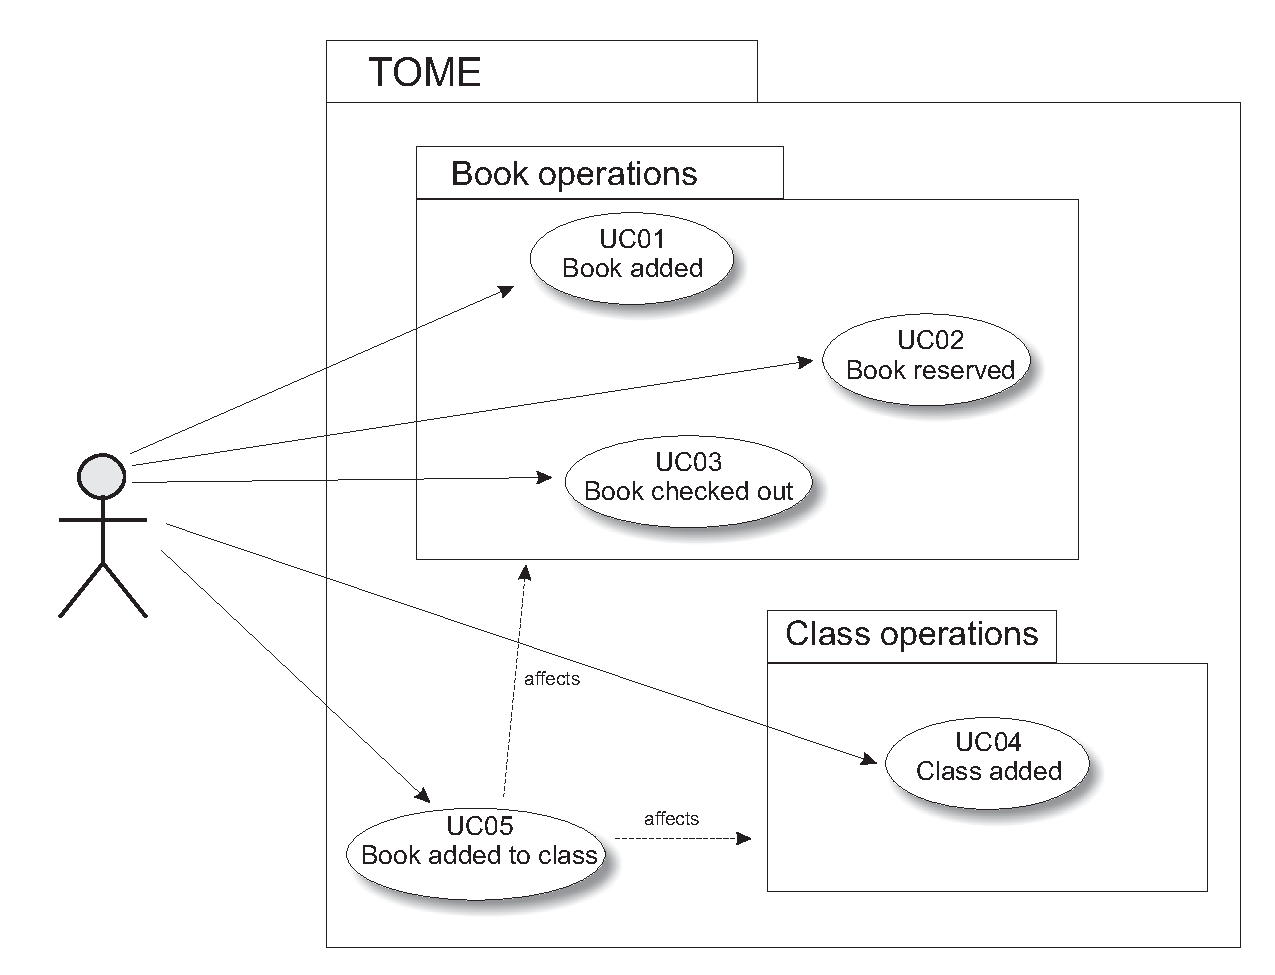
\includegraphics[width=\textwidth]{GraphicalUseCaseDiagram}
	\caption{Use Case Diagram}
	\label{usecase}
\end{figure}
\subsection{Business Use Cases}
This section documents the complete business scenarios within the scope of this project.


\subsubsection{UC01: Book Added}
\paragraph{Description}
This scenario happens when a patron donates a book to the TOME on their floor.  The book information must be entered in the system, and the book must be assigned a unique ID number by the system.
\paragraph{Actors}
TOMEkeeper and (indirectly) Patron
\paragraph{Preconditions}
\begin{enumerate}
	\item The TOMEkeeper must have an account
	\item The TOMEkeeper must be logged in
\end{enumerate}
\paragraph{Use Case Text}
\begin{enumerate}
	\item Patron requests to donate a book
	\item TOMEkeeper enters the book information into the system
	\item TOME assigns a book ID and presents the book information page
\end{enumerate}
\paragraph{Alternate Courses}
None.
\paragraph{Extends}
None.
\paragraph{User Interfaces}
ID0005.
\paragraph{Constraints}
None.
\paragraph{Questions}
None.
\paragraph{Notes}
None.
\paragraph{Source Documents}
None.


\subsubsection{UC02: Book Reserved}
\paragraph{Description}
This scenario happens when a patron requests that a book be reserved for them for a particular semester.
\paragraph{Actors}
TOMEkeeper and (indirectly) Patron
\paragraph{Preconditions}
\begin{enumerate}
	\item The TOMEkeeper must have an account
	\item The TOMEkeeper must be logged in
\end{enumerate}
\paragraph{Use Case Text}
\begin{enumerate}
	\item Patron sends their class list to the TOMEkeeper
	\item TOMEkeeper enters the class information into the system
	\item TOME determines what book reservations can be made, makes them, and notifies the patron via email
\end{enumerate}
\paragraph{Alternate Courses}
None.
\paragraph{Extends}
None.
\paragraph{User Interfaces}
ID0004.
\paragraph{Constraints}
None.
\paragraph{Questions}
None.
\paragraph{Notes}
None.
\paragraph{Source Documents}
None.

\subsubsection{UC03: Book Checked Out}
\paragraph{Description}
This scenario happens when a patron requests that a book be checked out for a semester
\paragraph{Actors}
TOMEkeeper and (indirectly) Patron
\paragraph{Preconditions}
\begin{enumerate}
	\item The TOMEkeeper must have an account
	\item The TOMEkeeper must be logged in
\end{enumerate}
\paragraph{Use Case Text}
\begin{enumerate}
	\item Patron requests that the book be checked out.  This may have already been done in the form of a reservation, or the patron can make the request without a previous reservation
	\item The TOMEkeeper checks a specific instance of the book out to the patron, and the system logs that checkout
\end{enumerate}
\paragraph{Alternate Courses}
None.
\paragraph{Extends}
None.
\paragraph{User Interfaces}
ID0007.
\paragraph{Constraints}
None.
\paragraph{Questions}
None.
\paragraph{Notes}
None.
\paragraph{Source Documents}
None.

\subsubsection{UC04: Class Added}
\paragraph{Description}
This scenario happens when a TOMEkeeper adds a class to the system
\paragraph{Actors}
TOMEkeeper
\paragraph{Preconditions}
\begin{enumerate}
	\item The TOMEkeeper must have an account
	\item The TOMEkeeper must be logged in
\end{enumerate}
\paragraph{Use Case Text}
\begin{enumerate}
	\item The TOMEkeeper finds a class that needs to be added to the system
	\item The TOMEkeeper adds the class to the system
\end{enumerate}
\paragraph{Alternate Courses}
None.
\paragraph{Extends}
None.
\paragraph{User Interfaces}
ID0006.
\paragraph{Constraints}
None.
\paragraph{Questions}
None.
\paragraph{Notes}
None.
\paragraph{Source Documents}
None.

\subsubsection{UC05: Book Added To Class}
\paragraph{Description}
This scenario happens when a TOMEkeeper adds a book to a class that is already listed in the system.
\paragraph{Actors}
TOMEkeeper
\paragraph{Preconditions}
\begin{enumerate}
	\item The TOMEkeeper must have an account
	\item The TOMEkeeper must be logged in
	\item The class to be added to must already exist within the system
\end{enumerate}
\paragraph{Use Case Text}
\begin{enumerate}
	\item The TOMEkeeper finds a book that needs to be added to a particular class
	\item The TOMEkeeper navigates to the class information page
	\item The TOMEkeeper adds the book to the class
\end{enumerate}
\paragraph{Alternate Courses}
None.
\paragraph{Extends}
None.
\paragraph{User Interfaces}
ID0003.
\paragraph{Constraints}
None.
\paragraph{Questions}
None.
\paragraph{Notes}
None.
\paragraph{Source Documents}
None.

\section{Business Domain Model}
The business domain model provides a listing of the modules contained in the project and how they work together.  This framework gives the project team a high-level guide to use in developing the project.
\subsection{Business Class Diagram}
Figure~\ref{BusinessModelDiagram} shows a graphical representation of the business classes involved in the TOME system.
\begin{figure}[h]
	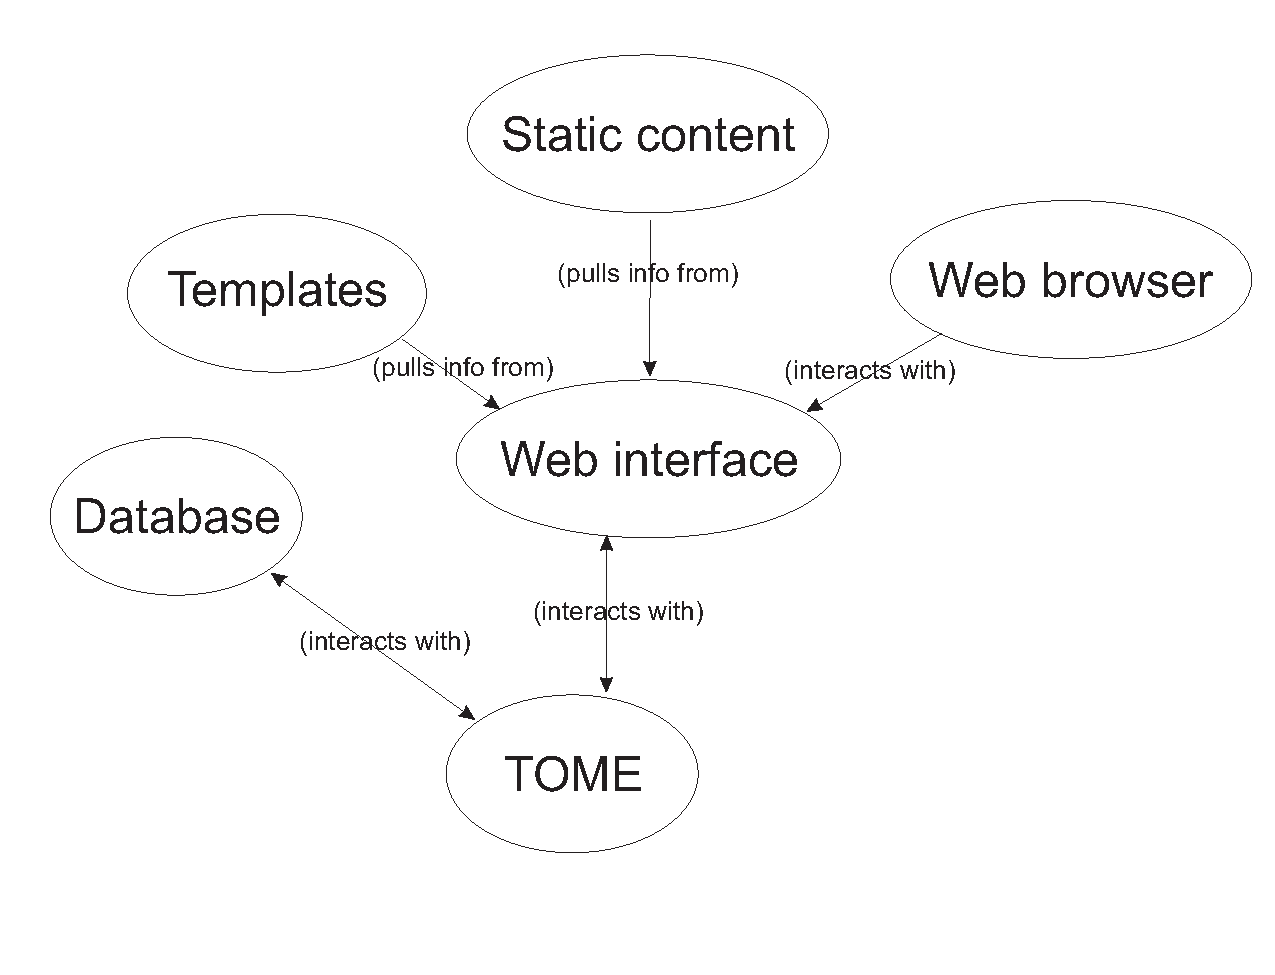
\includegraphics[width=\textwidth]{BusinessModelDiagram}
	\caption{Business Class Diagram}
	\label{BusinessModelDiagram}
\end{figure}
\newpage
\subsection{Business Object Definitions}
\subsubsection{TOME}
\begin{longtable}{|p{.25\textwidth}|p{.75\textwidth}|}
	\hline
	\textbf{Description} & TOME is the core module that processes database requests from the Web Interface.\\
	\hline
	\textbf{Attributes} & TOME contains all the methods used for interacting with the database as well as processing template files.\\
	\hline
	\textbf{Responsibilities} & TOME is responsible for all database communication, all template processing, all error handling, and any other ``core'' functionality\\
	\hline
	\textbf{Business Rules} & TOME has dependencies on many Perl modules (listed in the install document that can be located by referencing Section~\ref{references}).  These must be installed before TOME will function properly.\\
	\hline
\end{longtable}
Figure~\ref{TOMESequenceDiagram} is an example sequence of events involving TOME.
\begin{figure}[h]
	\centering
	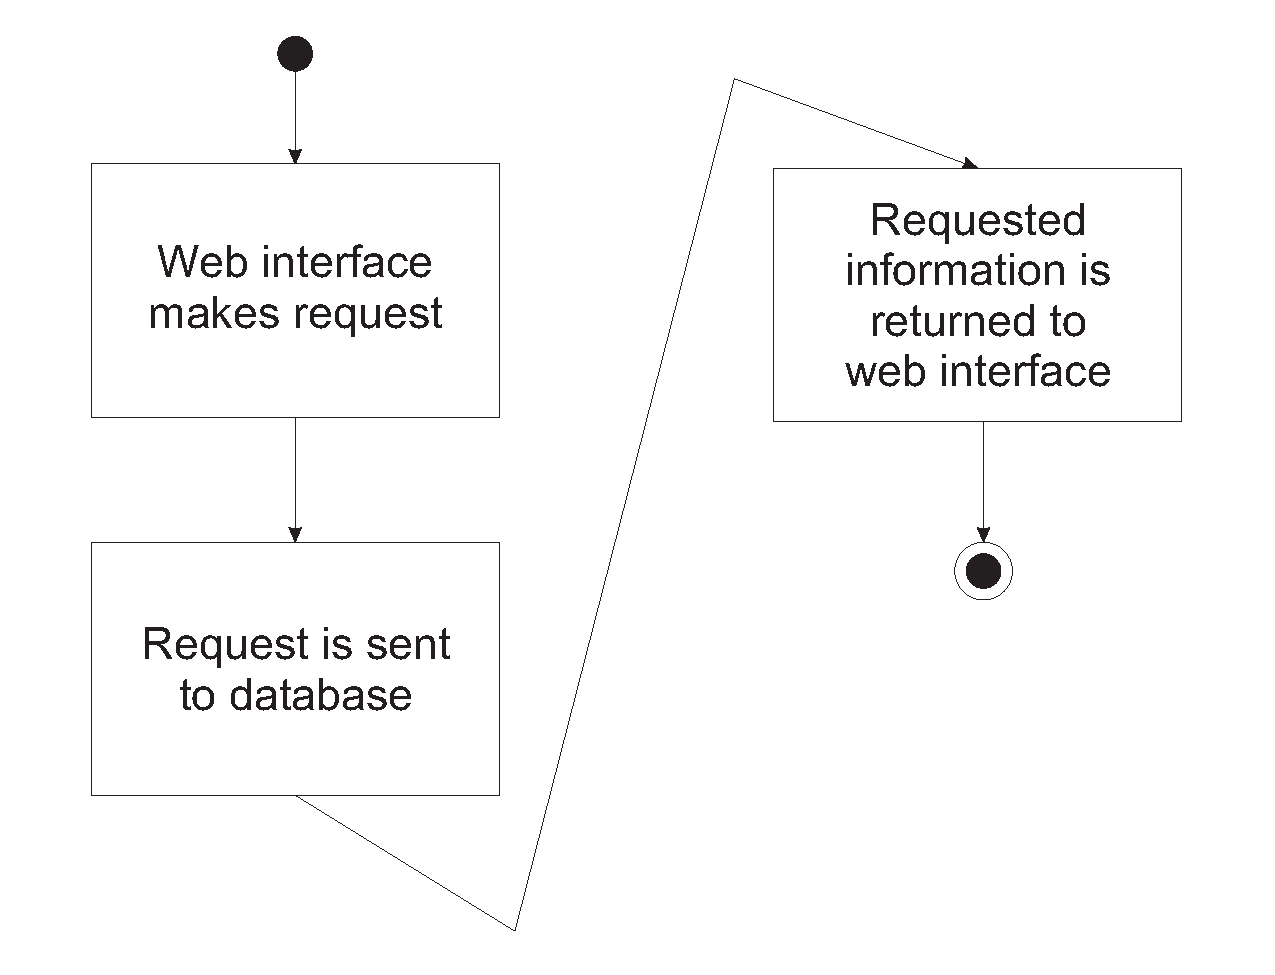
\includegraphics[width=.5\textwidth]{TOMESequenceDiagram}
	\caption{TOME Sequence Diagram}
	\label{TOMESequenceDiagram}
\end{figure}


\subsubsection{Database}
\begin{longtable}{|p{.25\textwidth}|p{.75\textwidth}|}
	\hline
	\textbf{Description} & The database is where all the information for TOME is stored.  The current implementation uses PostgreSQL for the database and DBI for all database interactions. \\
	\hline
	\textbf{Attributes} & All TOME data is stored in the database.  See Section~\ref{tomedbsection} for more details. TOME communicates with the database to retrieve, insert, and update all data for the system.\\
	\hline
	\textbf{Responsibilities} & The database is responsible for maintaining a consistent state for all data at all times. \\
	\hline
	\textbf{Business Rules} & PostgreSQL must be installed before the system will be functional. \\
	\hline
\end{longtable}
Figure~\ref{DatabaseSequenceDiagram} is an example sequence of events involving the database.
\begin{figure}[h]
	\centering
	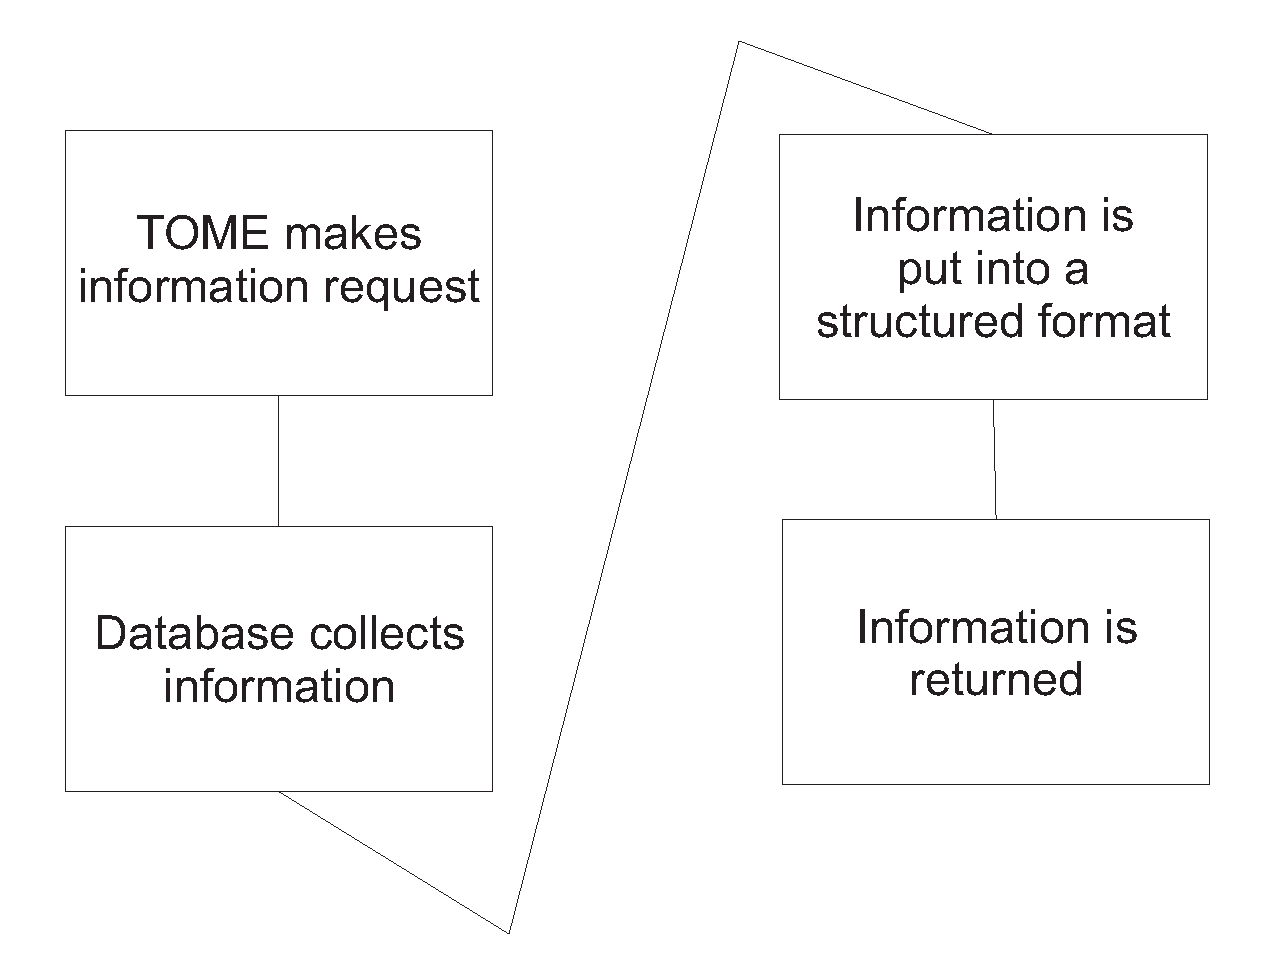
\includegraphics[width=.5\textwidth]{DatabaseSequenceDiagram}
	\caption{Database Sequence Diagram}
	\label{DatabaseSequenceDiagram}
\end{figure}


\subsubsection{Web Interface}
\begin{longtable}{|p{.25\textwidth}|p{.75\textwidth}|}
	\hline
	\textbf{Description} & The Web Interface forms the connection between the Database and the Templates.  It processes information that TOME retrieves from the Database and sends it to the templates.  It also processes user requests and sends them to TOME.\\
	\hline
	\textbf{Attributes} & The Web Interface contains all methods related to interacting with the user via CGI.\\
	\hline
	\textbf{Responsibilities} & The Web Interface is responsible for taking any data the user submits, verifying its validity, and submitting it to TOME to be run through the Database.  It is also responsible for taking information that TOME retrieved from the Database and preparing it for the templates to use.\\
	\hline
	\textbf{Business Rules} & The Web Interface depends on a number of Perl modules (see the Install document referenced in Section~\ref{references}) and these must be installed before it will be functional.\\
	\hline
\end{longtable}
\newpage
Figure~\ref{WebInterfaceSequenceDiagram} is an example sequence of events involving the Web Interface.
\begin{figure}[h]
	\centering
	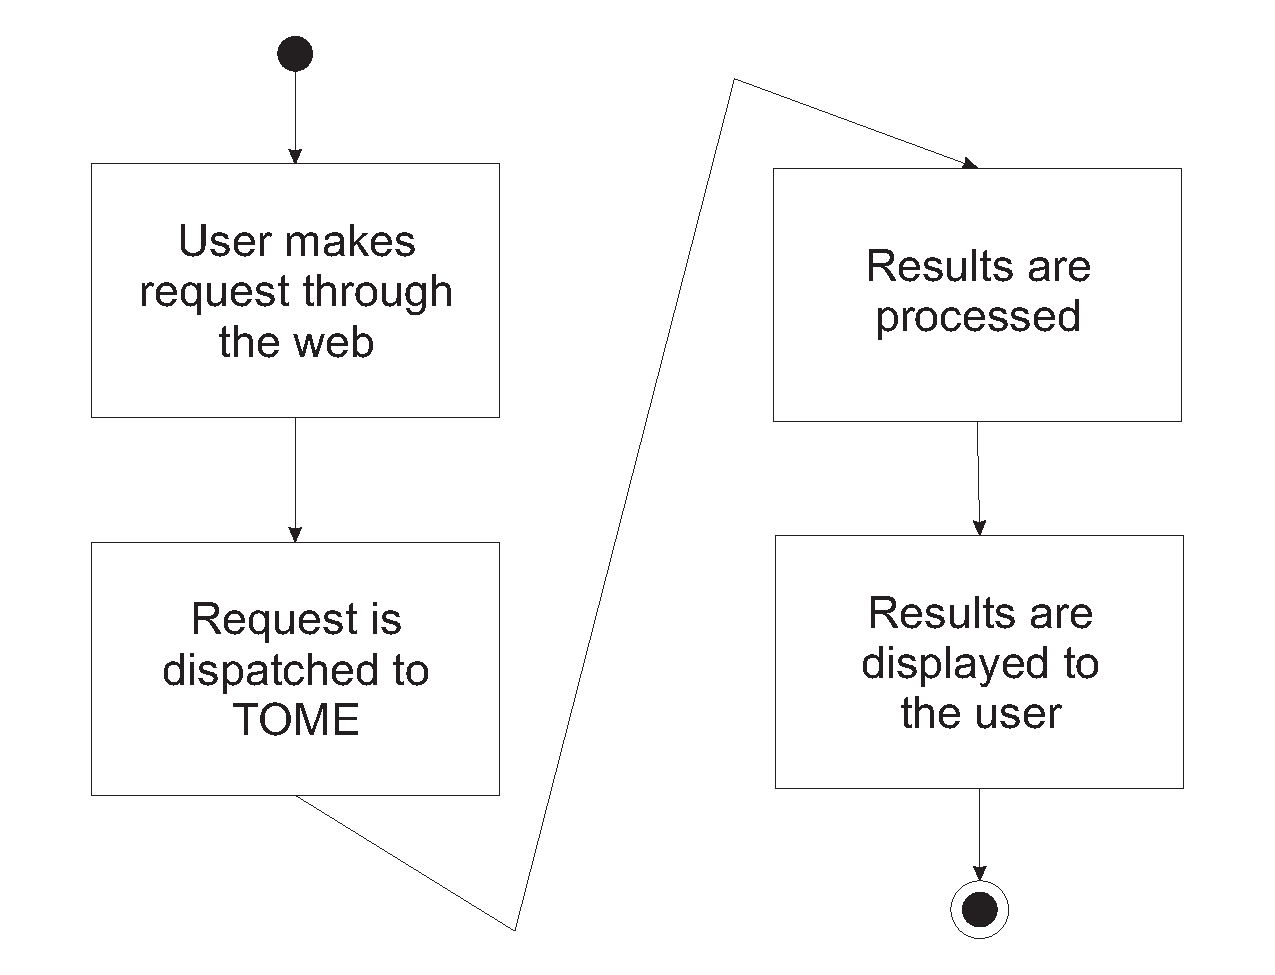
\includegraphics[width=.5\textwidth]{WebInterfaceSequenceDiagram}
	\caption{Web Interface Sequence Diagram}
	\label{WebInterfaceSequenceDiagram}
\end{figure}

\subsubsection{Templates}
\begin{longtable}{|p{.25\textwidth}|p{.75\textwidth}|}
	\hline
	\textbf{Description} & Templates form the basis for the look and feel of the web interface.  They do not give any functionality in and of themselves, but are a way to display information that is given by the Web Interface\\
	\hline
	\textbf{Attributes} & Templates have no methods, they only contain the data that determines how information is formatted and displayed.\\
	\hline
	\textbf{Responsibilities} & The templates must take information that is given to them by the Web Interface and format it.  In the process of formatting that information, they may request more information through a callback mechanism.\\
	\hline
	\textbf{Business Rules} & The templates need to be XHTML and CSS compliant. \\
	\hline
\end{longtable}
Figure~\ref{TemplateSequenceDiagram} is an example sequence of events involving template generation.
\begin{figure}[h]
	\centering
	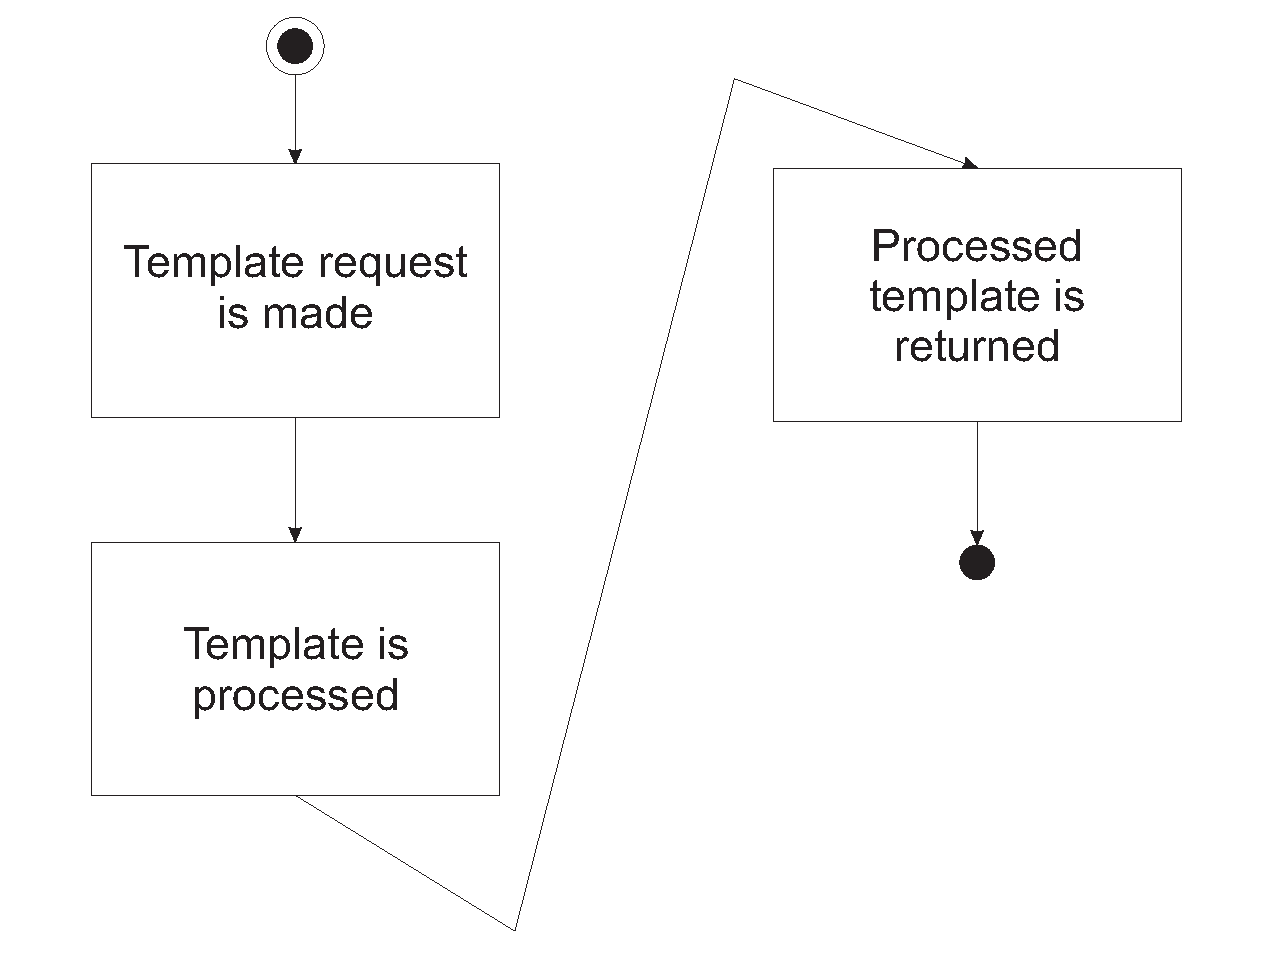
\includegraphics[width=.5\textwidth]{TemplateSequenceDiagram}
	\caption{Template Sequence Diagram}
	\label{TemplateSequenceDiagram}
\end{figure}

\section{User Interface Requirements Specification}
\subsection{User Interface}
The interface is entirely web-based.  Interaction with the Web Interface, which is displayed through templates accesses the TOME system which interacts with the Database.
\subsection{Navigation Model}
Figure~\ref{NavigationDiagram} graphically displays how the user interacts with TOME through the Web Interface.
\begin{figure}[h]
	\centering
	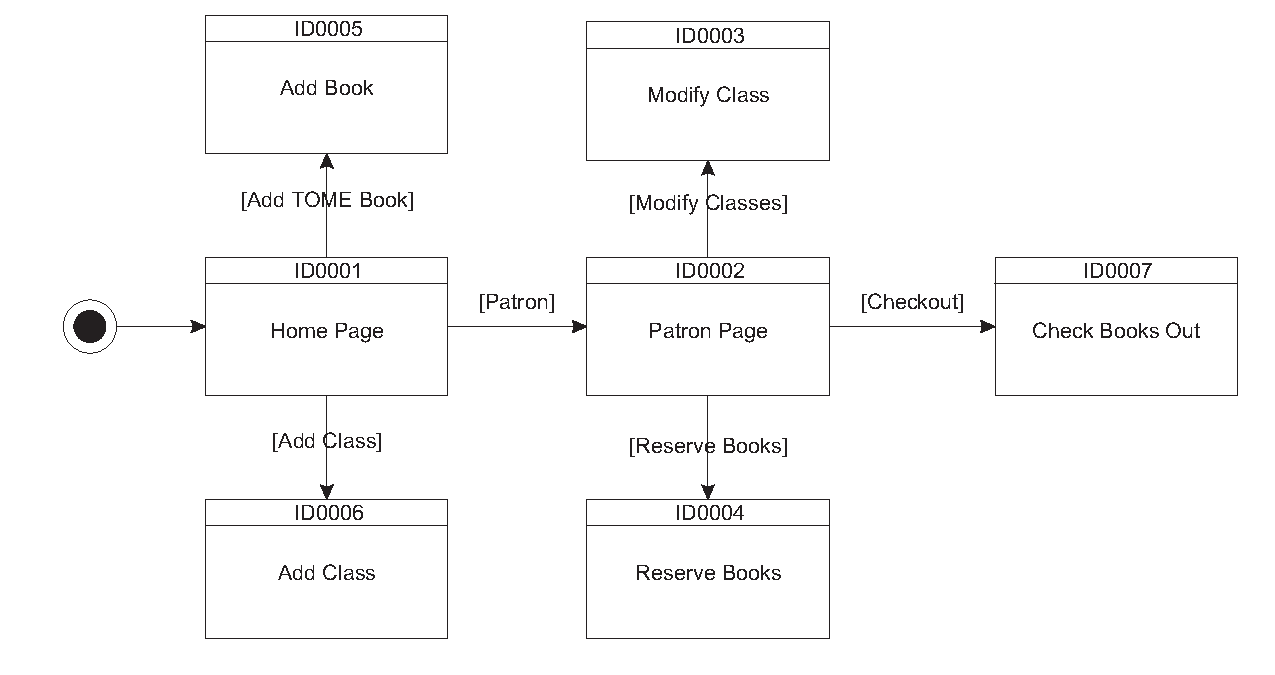
\includegraphics[width=\textwidth]{NavigationDiagram}
	\caption{Template Sequence Diagram}
	\label{NavigationDiagram}
\end{figure}
\subsection{Screens}
\begin{longtable}{|p{.25\textwidth}|p{.75\textwidth}|}
	\hline
	\textbf{Screen ID} & \textbf{Description} \\
	\hline
	ID0001 & Home Page \\
	\hline
	ID0002 & Patron Page \\
	\hline
	ID0003 & Modify Class \\
	\hline
	ID0004 & Reserve Books \\
	\hline
	ID0005 & Add Book \\
	\hline
	ID0006 & Add Class \\
	\hline
	ID0007 & Check Books Out \\
	\hline
\end{longtable}
\newpage
\subsection{View Definitions}
\subsubsection{Home Page}
\begin{longtable}{|p{.25\textwidth}|p{.75\textwidth}|}
	\hline
	\textbf{View Title} & TOME \\
	\hline
	\textbf{Number} & ID0001 \\
	\hline
	\textbf{Description} & This is the main home page for TOME and contains links to all major functions.  It also displays basic information about the status of the system such as the current semester and the current user that is logged in. \\
	\hline
	\textbf{Scenario References} & None.\\
	\hline
\end{longtable}

\newpage
\subsubsection{Patron Page}
\begin{longtable}{|p{.25\textwidth}|p{.75\textwidth}|}
	\hline
	\textbf{View Title} & Patron Page \\
	\hline
	\textbf{Number} & ID0002 \\
	\hline
	\textbf{Description} & This page displays information about the currently selected patron such as books currently checked out, books reserved, and classes for the current semester.  It serves as a starting point for many of the patron-related tasks.\\
	\hline
	\textbf{Scenario References} & None.\\
	\hline
\end{longtable}

\subsubsection{Modify Class}
\label{modifyclass}
\begin{longtable}{|p{.25\textwidth}|p{.75\textwidth}|}
	\hline
	\textbf{View Title} & Class Information Page\\
	\hline
	\textbf{Number} & ID0003 \\
	\hline
	\textbf{Description} & From the class information page, information can be modified about a class.  Comments can be made, books for the class can be added, deleted, and modified, and other maintenance work can be done.\\
	\hline
	\textbf{Scenario References} & UC05.\\
	\hline
\end{longtable}

\subsubsection{Reserve Books}
\begin{longtable}{|p{.25\textwidth}|p{.75\textwidth}|}
	\hline
	\textbf{View Title} & Reserve Books\\
	\hline
	\textbf{Number} & ID0004 \\
	\hline
	\textbf{Description} & From the patron information page, classes can be added for that patron.  Once a class information table is built up, the TOMEkeeper can start to reserve books for that semester for the patron.  This process will happen in steps where information about a class and its book associations is presented to the TOMEkeeper, and the TOMEkeeper makes the appropriate selections.  After the selections are made, the books are reserved and the patron is emailed a notification of what all happened.\\
	\hline
	\textbf{Scenario References} & UC02.\\
	\hline
\end{longtable}

\subsubsection{Add Book}
\begin{longtable}{|p{.25\textwidth}|p{.75\textwidth}|}
	\hline
	\textbf{View Title} & Add TOME Book\\
	\hline
	\textbf{Number} & ID0005 \\
	\hline
	\textbf{Description} & When a patron desires to add a book, this is the interface that will be shown.  From this page, the TOMEkeeper will enter basic information about the book such as the ISBN and which patron donated the book.  If TOME is unaware of the ISBN, the TOMEkeeper will be presented with a form to fill out the rest of the information about the book.\\
	\hline
	\textbf{Scenario References} & UC01.\\
	\hline
\end{longtable}

\subsubsection{Add Class}
\begin{longtable}{|p{.25\textwidth}|p{.75\textwidth}|}
	\hline
	\textbf{View Title} & Add Class\\
	\hline
	\textbf{Number} & ID0006 \\
	\hline
	\textbf{Description} & If a TOMEkeeper desires to add a class to the system, they will use this interface.  Adding a class is as simple as entering in the class ID and a name for the class.  All class information is added through the interface defined in Section~\ref{modifyclass}.\\
	\hline
	\textbf{Scenario References} & UC04.\\
	\hline
\end{longtable}

\subsubsection{Check Books Out}
\begin{longtable}{|p{.25\textwidth}|p{.75\textwidth}|}
	\hline
	\textbf{View Title} & Check Book Out\\
	\hline
	\textbf{Number} & ID0007 \\
	\hline
	\textbf{Description} & When it comes time to actually check a physical instance of a book out, this is the interface that will be used.  The TOMEkeeper can either change an existing reservation into a checkout, or they can specify the exact book to be checked out.  After this is accomplished, the Patron can take the book for the semester.\\
	\hline
	\textbf{Scenario References} & UC03.\\
	\hline
\end{longtable}

\section{Non-Functional Requirements Specification}
The Business Scenario Model only represents part of the full set of requirements.  Although the Business Scenario Model represents the functional requirements that are included in the project, there are many intangible requirements that haven’t been covered.  The purpose of this section is to document the non-functional requirements of TOME.
\subsection{Overview}
The non-functional requirements outlined in this section include the technologies needed to allow TOME to run, capacity planning strategies, and operational parameters.
\subsection{Enabling Technologies}
\subsubsection{Target Hardware and Hardware Interfaces}
TOME is a reasonably lightweight application.  It is targeted to run on any server-class computer.  If the computer is fast enough to run Apache, PostgreSQL, and Perl, it is fast enough for TOME.  Of course, the more users that access the system, the faster and bigger the server will have to be.
\subsubsection{Target Development Environment}
Development machines will utilize Vim, PostgreSQL, Subversion, and Perl on a Linux platform.
\subsubsection{System Interfaces}
TOME is a very high-level application, and as such will not have any direct interfaces to the system itself.  Apache will handle all network communication with the user, and PostgreSQL will handle all data storage.
\subsection{Capacity Planning}
\subsubsection{Traffic Volumes over Time}
Because TOME is a web application, its traffic is very ``bursty.''  TOME will have a high draw on system resources during the time a request is handled, but after the request has been handled there is no load on the system.  So, TOME would go from a 0 when it isn't handling a request to a 1 when it is handling a request.
\subsubsection{User Populations and Locations}
TOME is intended to be used by TOMEkeepers.  They will primarily access the system using their personal computers on the floors they live.  However, during Christmas and Summer break, the TOMEkeepers will need to be able to access the system remotely.
\subsubsection{Permanent Storage}
The data that will be held is actually very small in volume.  It is all little chunks of text stored in a database.  A very large TOME installation will be on the order of tens of megabytes.
\subsection{Printing}
Any printing requirements will be handled by the user's web browser.  TOME has no intrinsic printing mechanisms.
\subsection{Network}
TOME has extensive network requirements, however they will be handled entirely by Apache and the host operating system.  TOME itself has no knowledge of network layout or transportation.
\subsection{Workstations}
Any workstation with a modern, standards-compliant web browser can be used to access TOME.
\subsection{Operational Parameters}
\subsubsection{Usability}
In order to be successful, TOME must be very user-friendly.  Its target audience is limited, so it doesn't need to be completely intuitive, but the TOMEkeeper's technical skills will range from the extremely proficient to the beginner.  To improve usability, the interface will be designed to make most operations as obvious as possible.  Care has been taken to make the workflows logical.  Also, training will be given to every new user.
\subsubsection{Reliability}
TOME must be extremely reliable.  The database is especially important.  Without the data, the system becomes useless, and without the system, hundreds of books could be misplaced.  In order to ensure the reliability of the database, extensive checks have been put in place to make sure the data is consistent at all times (see Section~\ref{tomedbsection} for details).

Nightly backups will be made of all the data in the system.  Restoring a backup after a catastrophic failure is as simple as reinstalling the system, and using the PostgreSQL data recovery tool to reload the database.
\subsubsection{Maintainability}
Maintainability is a large concern with TOME.  To improve maintainability, all code will be documented in both embedded POD and in overviews such as this one.  Development will always be done in a Subversion environment to ensure traceability of all changes.
\subsubsection{Portability}
TOME itself contains no platform-dependent code.  The install scripts do make assumptions about a Linux-based platform, but the install could be done manually on other platforms.  The bulk of the code is written to interface to other extremely portable libraries and systems such as PostgreSQL and CGI.
\section{Design Approach}
\subsection{Key Drivers}
Continued development of TOME will follow the basic pattern that already exists.  In some ways this is good because it will not need to be redesigned.  However, in some ways it can be a hindrance because the original design does not use objects as extensively as it could.  Even though it is less than ideal, it was determined that the benefit that would be gained by a complete redesign would not outweigh the cost in time lost on new development.
\subsection{Issues}
The primary issue was determining how to preserve orthogonality without changing too much of the existing design.  One of the best ideas was a way to separate template and interface interaction.  This is detailed in Section~\ref{templatecallbacks}.
\subsection{Solution Approach}
The solution that was chosen is to retain as much as possible while still aiming for orthogonality and development speed.  The system is broken into different modules that each have a well-defined problem domain and provide cohesion while minimizing coupling.
\section{Design}
\subsection{Overview}
TOME is subdivided into several components to promote orthogonality in design.  The three main components (or ``modules'') are TOME, TOME::Interface, and TOME::TemplateCallbacks.
\subsection{Assumptions}
None.
\subsection{Component Diagram}
Figure~\ref{ComponentDiagram} graphically depicts the component layout of the TOME system.
\begin{figure}[h]
	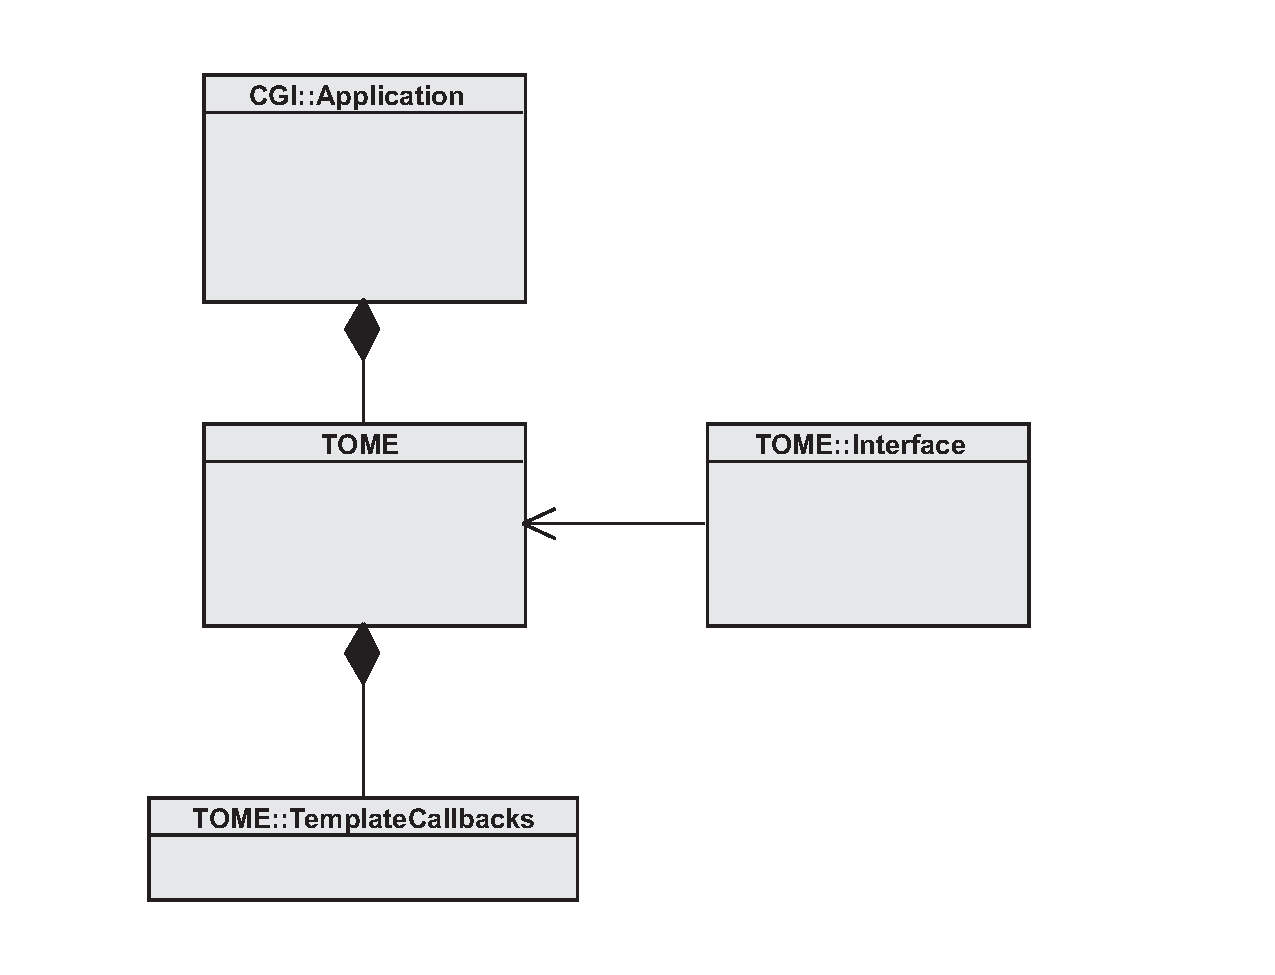
\includegraphics[width=\textwidth]{ComponentDiagram}
	\caption{Component Diagram}
	\label{ComponentDiagram}
\end{figure}
\subsection{Component Descriptions}
\subsubsection{TOME}
The purpose of this module is to provide database connectivity and all utility functions used by other parts of the program. Ideally, the TOME module shouldn't know anything about users and especially nothing about templates.
\subsubsection{TOME::Interface}
This is to control almost all interaction between the user and TOME. Nearly every method is a CGI::Application runmode, with the exception of a few helper subs. Ideally, TOME::Interface shouldn't know any details about the internal database structure or what things look like when they're displayed by the template.
\subsubsection{TOME::TemplateCallbacks}
\label{templatecallbacks}
Implements the TOME::TemplateCallbacks module. All templates are given a ``tome'' object that is an instantiation of this class. The idea is that when the template is given ID numbers of various things in the database (patrons, books, tomebooks, etc.) by TOME::Interface, the template can use this object to query the database through the TOME module and get string representations of the data. This module has the kinda funny place of knowing a little bit about both the template and the database. Most subs will probably just be wrappers of TOME subs, but if there is any additional data manipulation that needs to take place before the template (without crossing the line of actually doing template work), this is the place to do it. The reason this is separate from TOME is to give an extra layer of abstraction between the actual database calls and the template. Giving direct database access from inside a template is a thought too horrible to contemplate.
\section{Interfaces}
\subsection{Offered Services}
None.
\subsection{Internal Support Services}
Internal support services will be provided by TOME and TOME::TemplateCallbacks.
\subsection{External Services Required}
The services defined by the external libraries will be required.
\subsection{External Libraries Required}
In addition to Perl, Apache, PostgreSQL, and the Perl bindings for those technologies, the following Perl modules (and their dependencies) are required:
\begin{itemize}
	\item Template
	\item Template::Plugin::Comma
	\item Template::Plugin::CGI
	\item CGI::Application
	\item CGI::Application::Plugin::Session
	\item CGI::Application::Plugin::DBH
	\item CGI::Application::Plugin::HTMLPrototype
	\item CGI::Application::Plugin::ValidateRM (needs Compress::Zlib, even though CPAN doesn't show it as a prerequisite)
	\item CGI::Application::Plugin::Forward
	\item DateTime
	\item DateTime::Format::Pg
	\item SQL::Interpolate
	\item MIME::Lite
	\item Crypt::PasswdMD5
	\item DBD::Pg
\end{itemize}
\section{Test Strategy}
A framework will be created that is capable of running automated tests on all parts of the TOME system to ensure functionality and to prevent regression.  Tests will be broken up into the following categories: Database, Core, and Web Interface.  Tests will be made for all levels of functionality, starting from the database level, to check the consistency mechanisms and triggers, all the way up to simulating interaction with a user and a web browser.

Once completed, these tests will be run on a nightly basis.  They will be capable of creating a clean database and simulating a full range of activities.  All developers will be required to run and pass all tests before checking any new code in.
\section{Database Structure}
\label{tomedbsection}
The overall structure of the database can be seen in Figure~\ref{tomedb}.  In addition to the structure, there are also triggers that ensure the consistency of the database at all times.
\begin{figure}[h]
	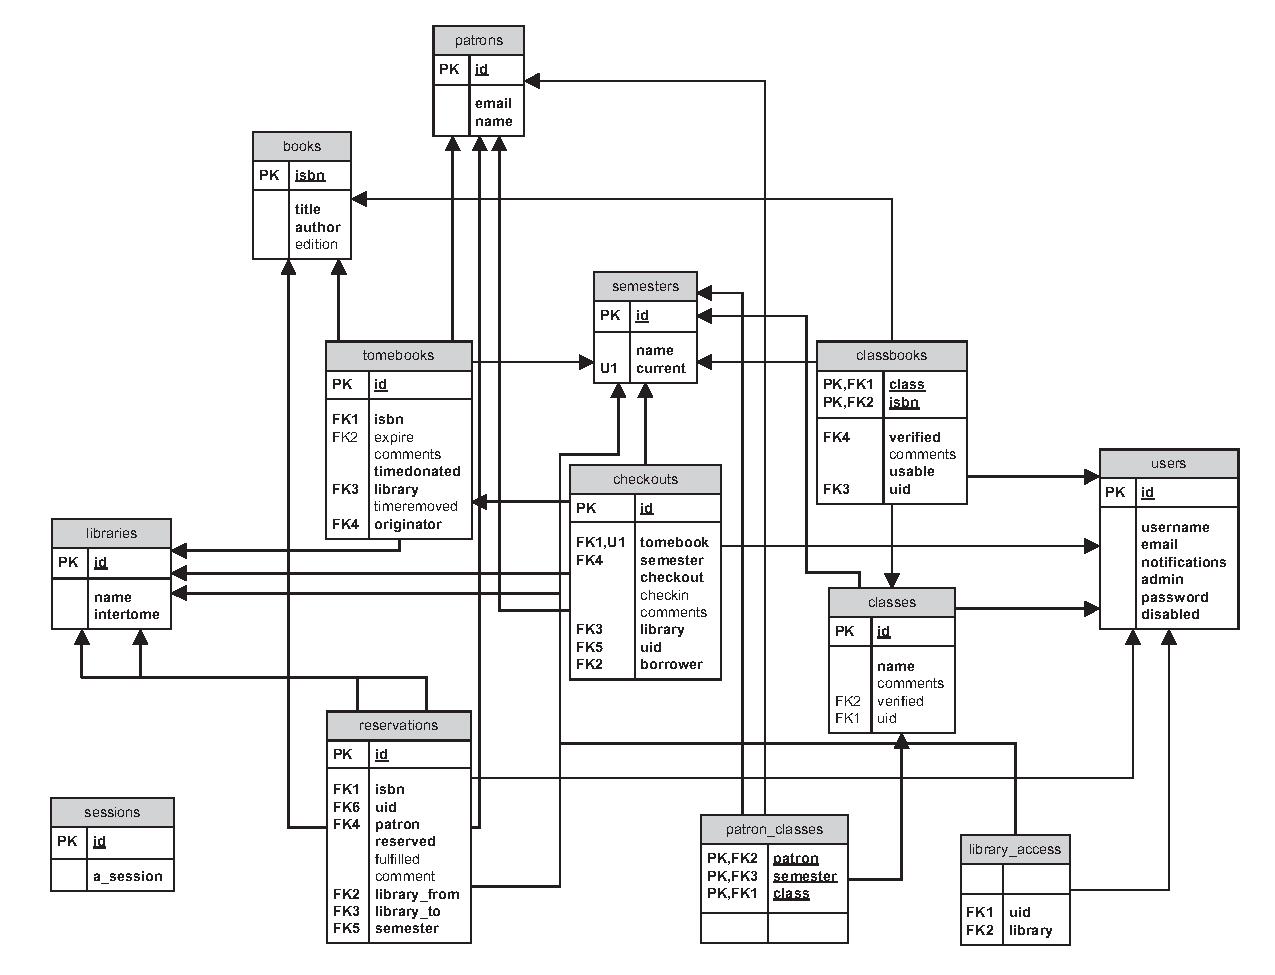
\includegraphics[width=\textwidth]{tomedb}
	\caption{Database Diagram}
	\label{tomedb}
\end{figure}
\end{document}

